\documentclass[tikz,border=12pt]{standalone}
\usetikzlibrary{arrows.meta,positioning}
\definecolor{pink}{HTML}{F72585}\definecolor{green}{HTML}{51CF66}\definecolor{amber}{HTML}{FCC419}
\definecolor{red}{HTML}{FF6B6B}\definecolor{blue}{HTML}{4DABF7}\definecolor{ink}{HTML}{E9ECEF}\definecolor{panel}{HTML}{211C1D}
\begin{document}
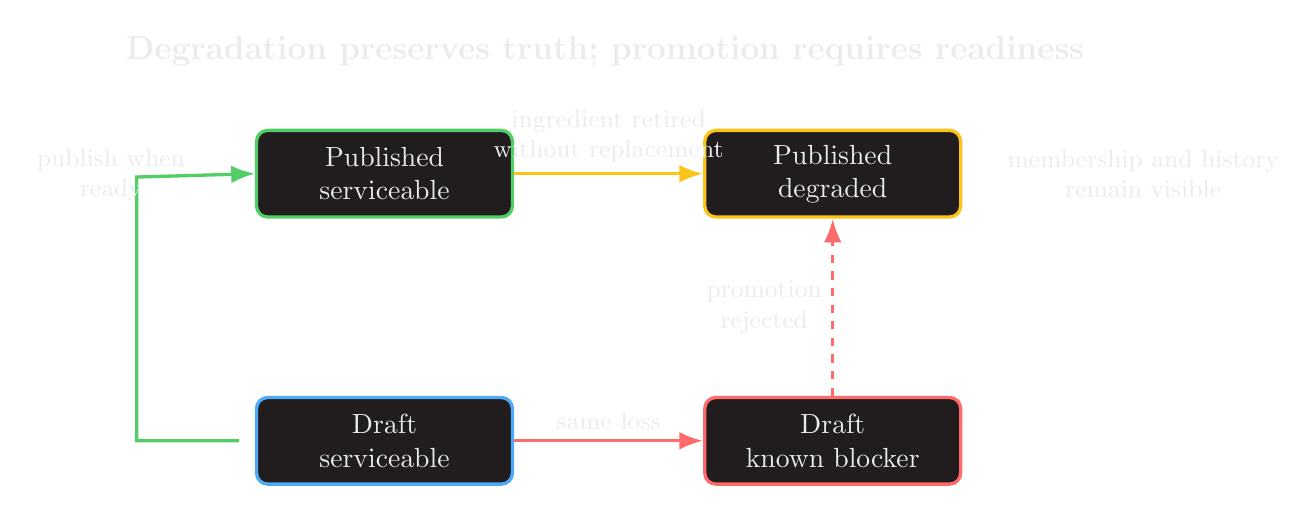
\begin{tikzpicture}[text=ink,state/.style={rounded corners=4pt,draw=blue,fill=panel,very thick,minimum width=3.25cm,minimum height=1.1cm,align=center},arrow/.style={-{Latex[length=3mm]},very thick},note/.style={font=\small,align=center,text=ink}]
 \node[state,draw=green] (published) {Published\\serviceable};
 \node[state,draw=amber,right=2.4cm of published] (degraded) {Published\\degraded};
 \draw[arrow,amber] (published)--node[above,note]{ingredient retired\\without replacement}(degraded);
 \node[note,right=.45cm of degraded] {membership and history\\remain visible};
 \node[state,below=2.25cm of published] (draft) {Draft\\serviceable};
 \node[state,draw=red,right=2.4cm of draft] (blocked) {Draft\\known blocker};
 \draw[arrow,red] (draft)--node[above,note]{same loss}(blocked);
 \draw[arrow,green] (draft.west)++(-.2,0)--++(-1.3,0)--++(0,3.35)--node[left,note]{publish when\\ready}(published.west);
 \draw[arrow,red,dashed] (blocked)--node[left,note]{promotion\\rejected}(degraded);
 \node[font=\bfseries\large,text=ink] at (2.8,1.55) {Degradation preserves truth; promotion requires readiness};
\end{tikzpicture}
\end{document}
